\chapter{Embedding machine learning models to process social media data in crisis management}

\section*{Introduction}
% * Done
This chapter takes a step back and looks at the information system as a whole.
In particular, it questions the place and stakes of machine learning in an information system for crisis management.
It is organized around the third research question identified initially in the first chapter:
\textit{What are the challenges faced by an information system dedicated to crisis management that uses machine learning models?}

\begin{figure}[htb]
    \centering
    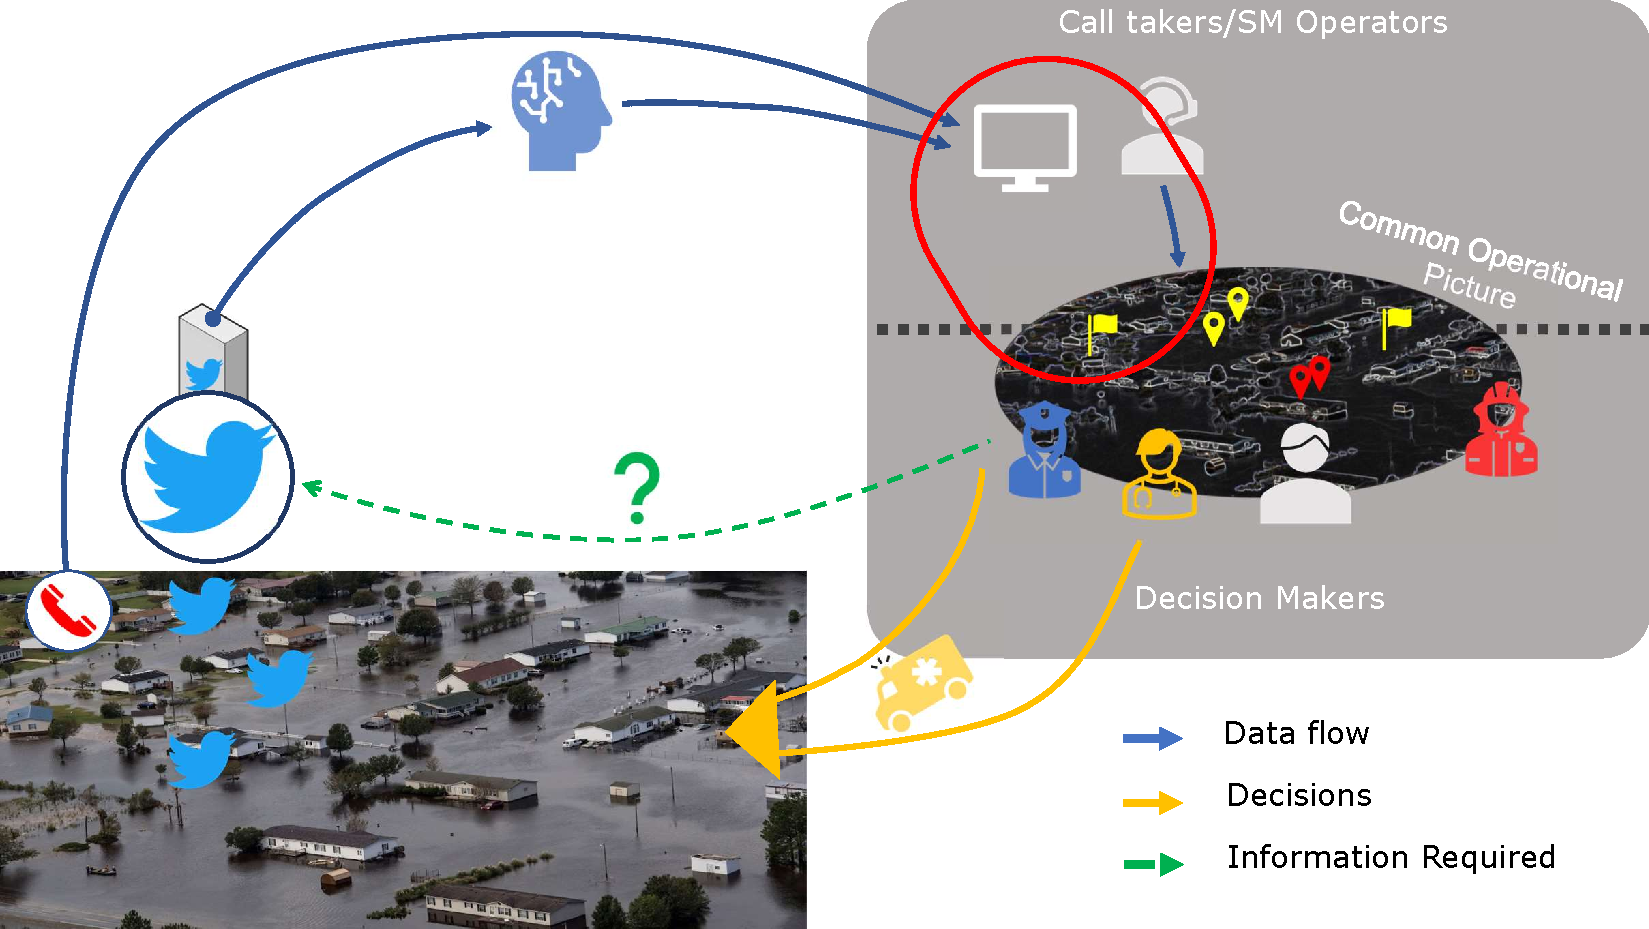
\includegraphics[width=\textwidth]{figures/chap-5/position-chapter.pdf}
    \caption{Position of this chapter with respect to the body of this manuscript.}
    \label{system:big-picture-manuscrit}
\end{figure}

Particularly, the previous chapters aimed to address a specific question: What kind of information are staff from emergency centers looking for on social media?
The previous chapter presented a method to automatically identify and retrieve entities within a text related considering decision-makers information expectations.
This solution, which differs from others by the level at which the text is processed, followed a widespread pattern of data processing used in crisis informatics.
This pattern is found in most of the systems reviewed in the second chapter.
It is composed of the following components and illustrated Figure~\ref{system:sm-processing}.

\begin{itemize}
    \item The \textbf{data collection} is a connector to the Application Programming Interface (API) of a
          social media platform, such as Twitter.
          This connector queries data in real-time from the platform according to a set of topics of interest.
    \item The \textbf{preprocessing} is in charge of normalizing the incoming data and preparing it for the processing aspect.
    \item The \textbf{processing} component provides information addressed to decision-makers, and that supports them in their operation, usually by enhancing their situational awareness of the ongoing event.
\end{itemize}

As a final step, some systems integrate a way to visualize the results through a dashboard, a geographical representation, etc.

\begin{figure}[htb]
    \centering
    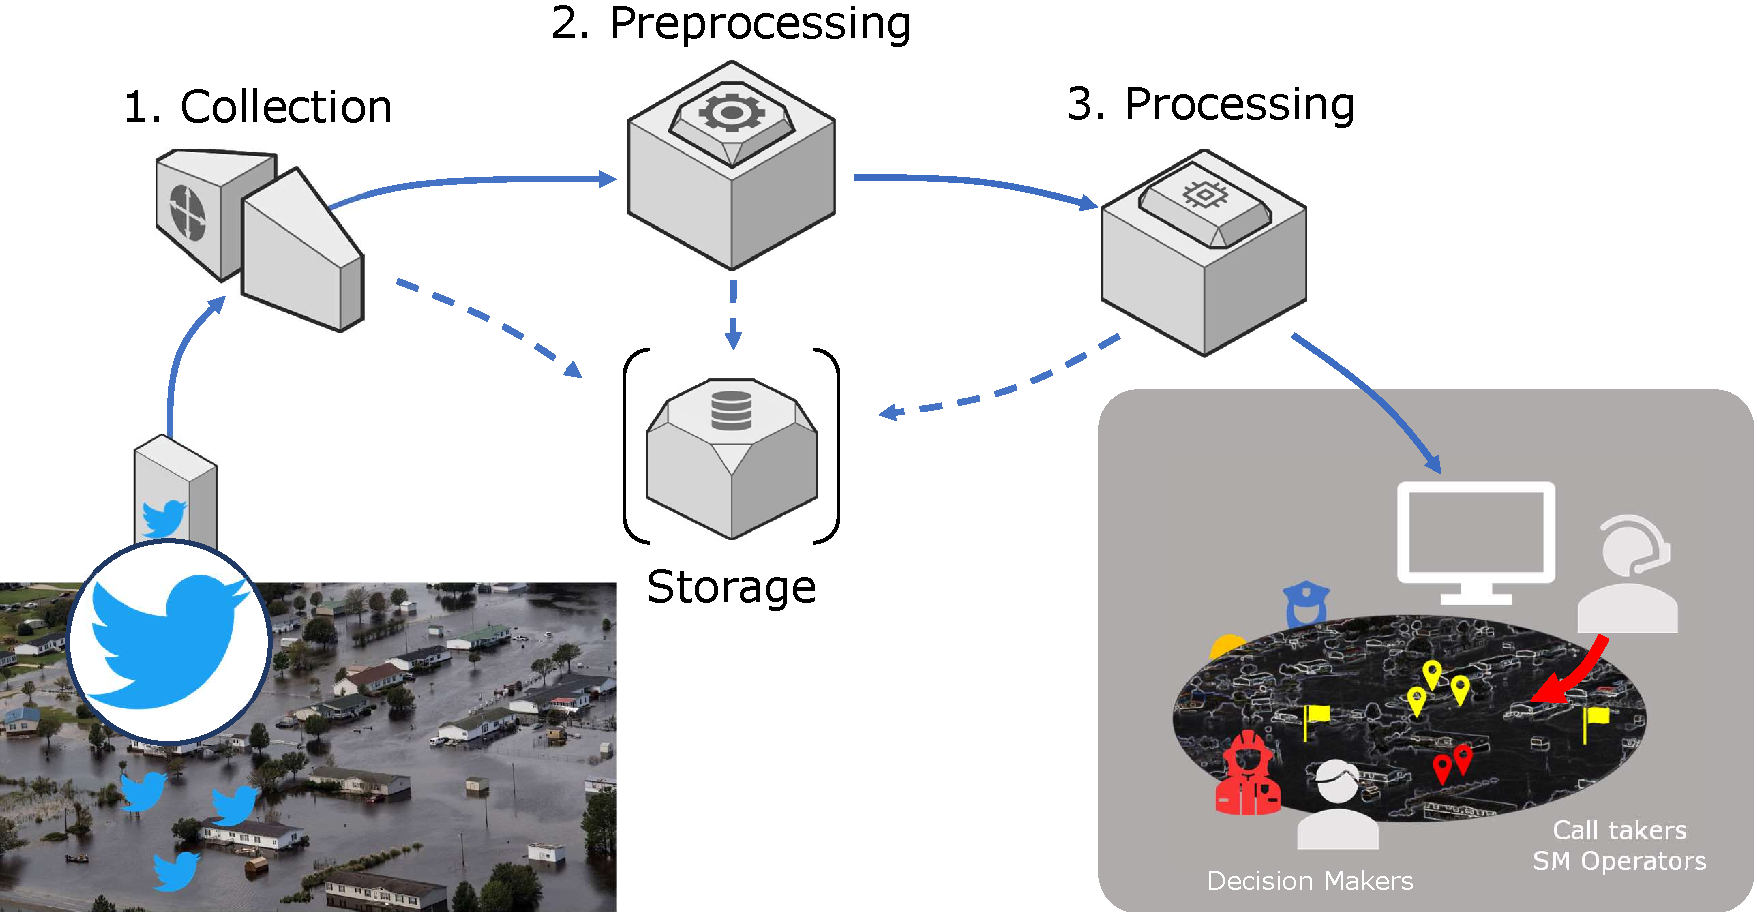
\includegraphics[width=\textwidth]{figures/chap-5/social-media-processing.pdf}
    \caption{Main pattern of steps in processing social media data used in previous attempts.}
    \label{system:sm-processing}
\end{figure}

The steps that compose this pattern are also found in systems that process images taken from citizens \parencite{alamImage4ActOnlineSocial2017} or drones \parencite{fanDisasterCityDigital2021}.
To improve performances or solve new challenges, systems built over time are different.
While they generally follow the previous pattern, they propose tweaks and differences to accommodate the added constraints.
There are, however, some elements that can be factorized:

\begin{itemize}
    \item The preprocessing of the data is a pipeline composed of sequential steps.
          For instance, model A may need lowered text as input, whereas model B needs the original text.
          Also, tokenizers, while often being different, are always present when one processes textual data.
    \item Processing and preprocessing are not uniquely paired. A processing component requires its appropriate preprocessor, but a preprocessor can be common to multiple processors.
    \item A processor can be appended to the preprocessing pipeline, and its result can be passed to another processor.
\end{itemize}

Hence, the data pipeline used to train and feed machine learning models with new data is a complex component of an information system.
However, previous works are often designed as data processing systems associated with visualization tools.
Few take into account the information system on which crisis management organizations rely.
From there, two organizations are possible.
The first is to make the information system coexist with the machine learning models and their associated visualization tools.
The second is to integrate the machine learning models within the information system.
The first option is easier to implement than the second one.
However, the second option allows greater agility in the processing of data and information.
However, several studies have shown the importance of better integration of the different sources of data and information in crisis management \parencite{comesBringingStructureDisaster2015,tapia2016scaling}.
This chapter details the challenges and opportunities offered by an information system that integrates the machine learning models needed to process social media data.
First, it presents the different challenges that such an information system presents.
The second section presents a general framework of the implementation with respect to the previous challenges identified.
The consecutive section describes the implementation of the social media module for the R-IO Suite software, using the previous framework.
The last section opens on the purpose of such systems: to provide information to decision-makers

\section{Challenges of the Information System - Operator - Machine Learning ecosystem}
% * Done
Machine learning methods have many applications for crisis response.
AI facilitates the processing of data and information by speeding by making it faster, allowing the processing of large volumes of data, etc.
In the context of disaster response, this ease of processing saves valuable time.
Nevertheless, some machine learning methods trade this additional efficiency at the price of transparency.
This section investigates the potential effects of a lack of transparency of information system components.
The first sub-section presents the problems encountered when designing an information system turned with the improvement of AS.
The second sub-section extends this reflection by looking specifically at the impact of machine learning.

\subsection{The SA daemons looming over the Information System}
Endsley, who originated the definition of situational awareness, identified various factors that prevented systems from providing maximum value to their users \parencite{endsleyDesigningSituationAwareness2016}.
The authors identify 8 "demons" (factors) in the design of the system that harms the Situational Awareness of the operators:

\begin{itemize}
    \item Attentional tunneling: fixating one set of information to the exclusion of the others.
    \item Requisite memory trap: over-reliance of the system on the operator's short memory.
    \item Workload, anxiety, fatigue, and other stressors
    \item Data overload
    \item Misplaced salience: misplaced warnings or signs that incorrectly catch the user attention
    \item Complexity creep: complex systems, cluttered of features, prevent the user from creating an accurate mental model
    \item Errant mental models: incorrect mental models ultimately lead to poor comprehension and projection
    \item Out-of-the-loop syndrome: automated systems sometimes do not completely inform the user
\end{itemize}

Additionally, they provide thoughts on the automation of resolving problems that involve a certain degree of Situation Awareness.
Automation can be responsible for three issues: (i) out of the loop syndrome, (ii) inaccurate understanding of the system by the operator, and (iii) diminishing return of decision support systems.
To prevent these caveats, the authors advise adaptive automation considering the user.
They organize their recommendations through eleven principles:

\begin{itemize}
    \item Automate only if necessary
    \item Use automation for assistance in carrying out routine actions rather than higher-level cognitive tasks
    \item Provide SA support rather than a decision
    \item Keep the operator in control and in the loop
    \item Avoid the proliferation of automation modes
    \item Make modes and system states salient
    \item Enforce automation consistency
    \item Avoid advanced queuing of tasks
    \item Avoid the use of information cueing
    \item Use methods of decision support that create human/system symbiosis
    \item Provide automation transparency
\end{itemize}

These insights are valuable in the design of an effective social media processing system for crisis response.
Yet, these principles will only be valuable to provide a better SA to the user of such a system.

\subsection{Is machine learning really coming to the rescue?}
% * Done
The use of machine learning in high-stakes systems is not without risk.
Many proposals have failed despite the best efforts of the teams to make the system successful.
Google proposed, for example, a service (Google Flu Trend) to follow the evolution of the flu in different countries.
The system relied on the searches performed by its users to predict future flu epidemics.
This system was discontinued in 2015 due to the large gap between predictions and reality, among other factors \textcite{lazerWhatWeCan2015,kandulaReappraisingUtilityGoogle2019}.
Another example is IBM's Watson Health AI system \parencite{stricklandIBMWatsonHeal2019}.
When this AI system launched in 2011, the system promised to revolutionize medical diagnostics.
A few years later, faced with the task's difficulty, IBM scaled back its medical ambitions for its AI.
IBM Watson Health has become an excellent AI librarian over time.
However, it still remains far away from its original promises.
As the article concludes: "The Watson Health story is a cautionary tale of hubris and hype.".
These two examples are unfortunately the only ones, and many other projects failed.
The available post mortems mostly point to a common problem: understanding the data used to train the machine learning models was simply insufficient.
Based on this conclusion, \textcite{sambasivanEveryoneWantsModel2021} conducted a qualitative study on the reasons for these failures.
Their main conclusion is that teams do not dedicate enough time to acquiring data of sufficient quality for the problem that the machine model is supposed to address.
Complex problems require datasets that reflect the complexity of the problem, allowing the machine learning model to identify the correct latent patterns.
Since the development of a machine learning model is sequential, each error or shortcoming in one of the steps affects the final result.
Based on this study and other concurrent projects, the same team summarized their findings in a guidebook of recommendations for products or systems that embed machine learning models \parencite{pairPeopleAIGuidebook2021}.
This guidebook has also been informed by the testimonials of hundreds of AI practitioners.
It is articulated around six axes that system or product designers should be mindful of:

\begin{itemize}
    \item User needs \& defining success—the AI needs to solve a problem.
          Automate unpleasant tasks, where there's a need for scale, and where people can define what the correct way to do it is.
          Augment high stake tasks or where people disagree on the "correct way" to do it.
    \item Data collection \& Evaluation—Data and its quality are of the utmost importance when building a machine learning model.
          Make sure that the users need to translate through the data.
    \item Mental Models—Build a system whose interface and functioning are familiar to the users.
          The differences should be highlighted at the onboarding stage (e.g., with a tutorial).
          Communicate the limitations of your system.
    \item Explainability \& Trust–Users can easily rely blindly on the system, especially in stressful situations.
          Thus, the system should provide as much as possible an indicator of the relevance of the prediction.
    \item Feedback \& Control—People like to remain in control, especially when the stakes are high.
          Therefore, the system must provide feedback to users so that they feel included in the decision-making process.
          Particularly the type of information that the AI should consider.
    \item Errors \& Graceful failure—Define failure and success according to your user's expectations (e.g., 60\% accuracy can be a success or a failure).
          The user should not be locked with a faulty AI, and the system should provide a path forward from failure.
\end{itemize}

Of the six recommendations made, many overlap with the previous recommendations formulated in \textcite{endsleyDesigningSituationAwareness2016}.
Both authors agree on certain aspects, such as keeping the user in the loop, highlighting the moments when the system is faulty, or creating a symbiosis between the human and the machine.
However, systems that rely on machine learning models do not seem to eliminate the previous daemons.
On the contrary, this approach brings new difficulties, which must be considered; otherwise, the whole system could be rendered unusable.
These insights will be used in the next sections.

\section{Information systems for disaster response: place and role of data and information}
% * Done
As presented in the first chapter, information systems (IS) are responsible for managing information in an organization.
They are organized around four functions:

\begin{itemize}
    \item Collect: they provide a gateway to users to ingest information;
    \item Process: information internal to the system can be processed to obtain newly derived information;
    \item Store: the IS is in charge of preserving the information it contains;
    \item Distribute: reverse function of the collection - the system proposes a way to exploit the ingested data.
\end{itemize}

These functions and the definition of the information system are rooted in the beginnings of computer science as a discipline.
If the different functions remain unchanged, the way to achieve them has changed through technological innovations.
Decision support systems, for instance, rely on artificial intelligence to deliver results to the users.
The first iterations of decision support systems relied on systems of rules encoded into the system.
The rules embed the knowledge of experts to deliver that knowledge automatically.
In recent years, the machine learning branch of artificial intelligence boomed.
This led to several outcomes.
First, information systems can automatically learn new rules directly from the data, without
the intervention of an expert, using machine learning models that learn these rules from the data they receive.
Secondly, and as a direct consequence of the first outcome, data management now occupies a larger role in the system.
Many systems have been developed using this approach, and some have been presented in the first chapter of this dissertation.
These systems are usually organized around five components:

\begin{itemize}
    \item One dedicated to \textit{data collection}
    \item A data \textit{preprocessing} component, in charge of normalizing the data in a format that suits the processing.
    \item A \textit{storage} component that stores the data and/or the result of the processing
    \item A \textit{processing} component, which is composed of the machine learning model, to which the collected are passed.
    \item A \textit{visualization} component
\end{itemize}

Other components can be, for instance, an interface to allow the general public to annotate the data during an event \parencite{imranAIDRArtificialIntelligence2014}.
The previous section has already presented the importance of data in a machine learning system.
The next subsection introduces a systematic solution to this issue through the MLOps approach.

\subsection{Machine learning models lifecycle: lessons from MLOps}
% * Done
Machine learning models undergo two phases in their existence within a system.
The first phase corresponds to the training of the model.
For this, the model takes as input the data previously collected and processed.
Once the training is complete, the performance of the model is then assessed to determine if it meets the expectations of the users.
The second phase consists in exploiting the trained model by providing it with new data from which we want to obtain a prediction.

During the second phase, the system is deployed to make predictions on incoming data.
\textcite[Chapter~1]{treveilIntroducingMLOps2020} highlight that this approach causes several issues.
First, contrary to the deployed model, the environment is constantly changing.
This phenomenon is called drifting and corresponds to a degradation of the performances, similar to wear.
This wear is not internal to the model (as we could conceive it for a machine in a factory) but to the environment in which the model evolves.
Thus, because of drifting, the models must be regularly updated.
In the case of crisis management, depending on the type of event and problem that one wants to solve, the model can be updated more frequently.
A flooding event, for instance, is a relatively well-known event.
It benefits from an extensive collection of data, so a model can be trained to recognize messages that are related to this event.
However, this model will not be able to identify more subtle sub-events resulting from an event cascade.
Another issue that \citeauthor{treveilIntroducingMLOps2020} highlights are the difficulty for a team to maintain machine learning models by hand.
Due to the above-mentioned environmental conditions, models have to be constantly monitored and adjusted in case of drifting.

This life cycle of machine learning models and their computing environment is at the heart of the Machine Learning Operations approach (MLOps).
This approach shares its acronym and philosophy with the DevOps methodology.
DevOps is the contraction of Development and Operations and aims to reduce the software development life cycle while maintaining high quality.
Inspired by this approach, Machine Learning Engineers developed a dedicated methodology for machine learning models.
However, the objective remains unchanged: reduce the time and complexity of machine learning models deployment.
The MLOps methodology is centered around the machine learning life cycle, illustrated Figure~\ref{system:ml-life-cycle} \parencite{treveilIntroducingMLOps2020,burkovMachineLearningEngineering2020}.

\begin{figure}[htb]
    \centering
    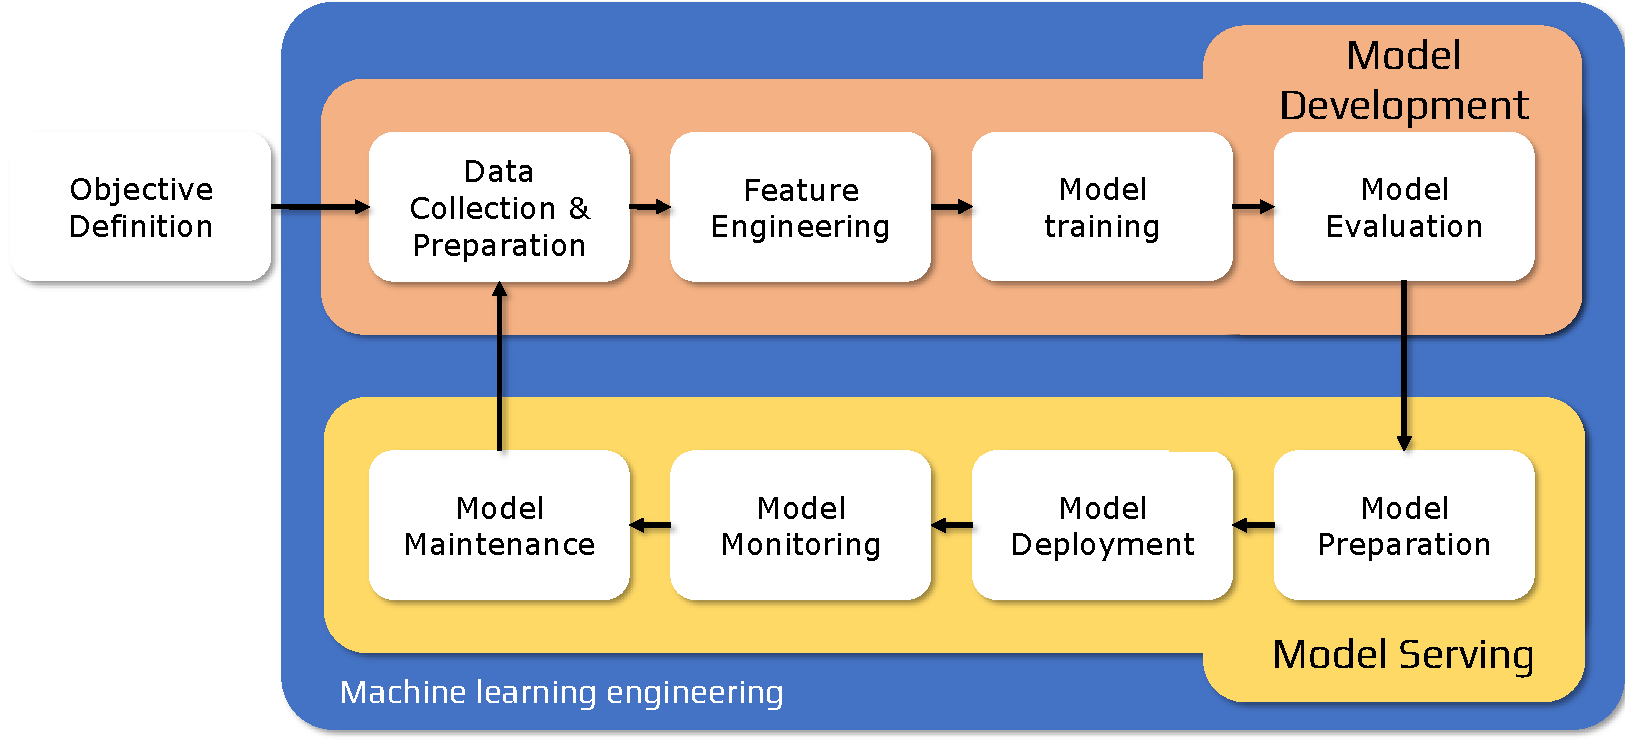
\includegraphics[width=\textwidth]{figures/chap-5/machine-learning-life-cycle.pdf}
    \caption{Life cycle of a machine learning project.}
    \label{system:ml-life-cycle}
\end{figure}

As mentioned in the previous section, the first steps, the objective definition, and the data collection are crucial to the success of the project as a whole.
Once quality data are retrieved and that the value offered is clear, features used by the machine learning model are extracted.
The model is then trained on the data and associated features.
This model is then evaluated to determine if it performs sufficiently to solve the users' problems.
These steps mark the end of the model development phase.
Onward, the model is deployed to serve its predictions.
The model preparation step sees quality testing and risk evaluation performed.
Once this step is clear, the model is packaged and deployed.
During its deployment, the model is monitored.
Ideally, its inputs and outputs are logged to capture the aforementioned environment changes.
The last step is model maintenance, where the model is updated according to the changes previously recorded.
One of the underlying motivations of the MLOps methodology is to perform as much as these steps automatically.
In the crisis management configuration, all steps up to the deployment of the model must be performed during the crisis preparation phase.
This way, the model is ready to be used during an event.
Suppose the model needs to be updated because it cannot provide the help that the operator expects.
In that case, the system must be designed to 1) notify the user of this fact 2) take into account the new entries recorded in order to update itself automatically.
This behavior must be transparent to the users of the system.

\subsection{Position and purpose of data and information in the system}
An information model that integrates machine learning models sees its information coexist with data.
\textcite{rainerIntroductionInformationSystems2021} define \textbf{data} as "an elementary description
of things, events, activities, and transactions that are recorded, classified, and stored,
but are not organized to convey any specific meaning".
As for \textbf{information}, the definition proposed is "[information] refers to data
that have been organized so that they have meaning and value to the recipient".
These definitions are related to those proposed by \textcite{ackoffDataWisdom1989} in the DIKW framework it proposes.
Although many systems have been developed by mixing the two concepts, the separation and organization of the two concepts allow for an overall vision conducive to discovering new opportunities.

The following research question guides the rest of this subsection: \textit{how do data and information management coexist within an information system based on machine learning models}?
The previous sections highlighted the importance of data within a system that contains machine learning models.
Consequently, the information system is no longer the only system present and paired with a Data System (DS).
Figure~\ref{system:ds-is-systems} provides an overview of the different components of both systems and how they organize to the machine learning life cycle.
The two following sub-sections discuss the place of data and information, respectively.

\begin{figure}[htb]
    \centering
    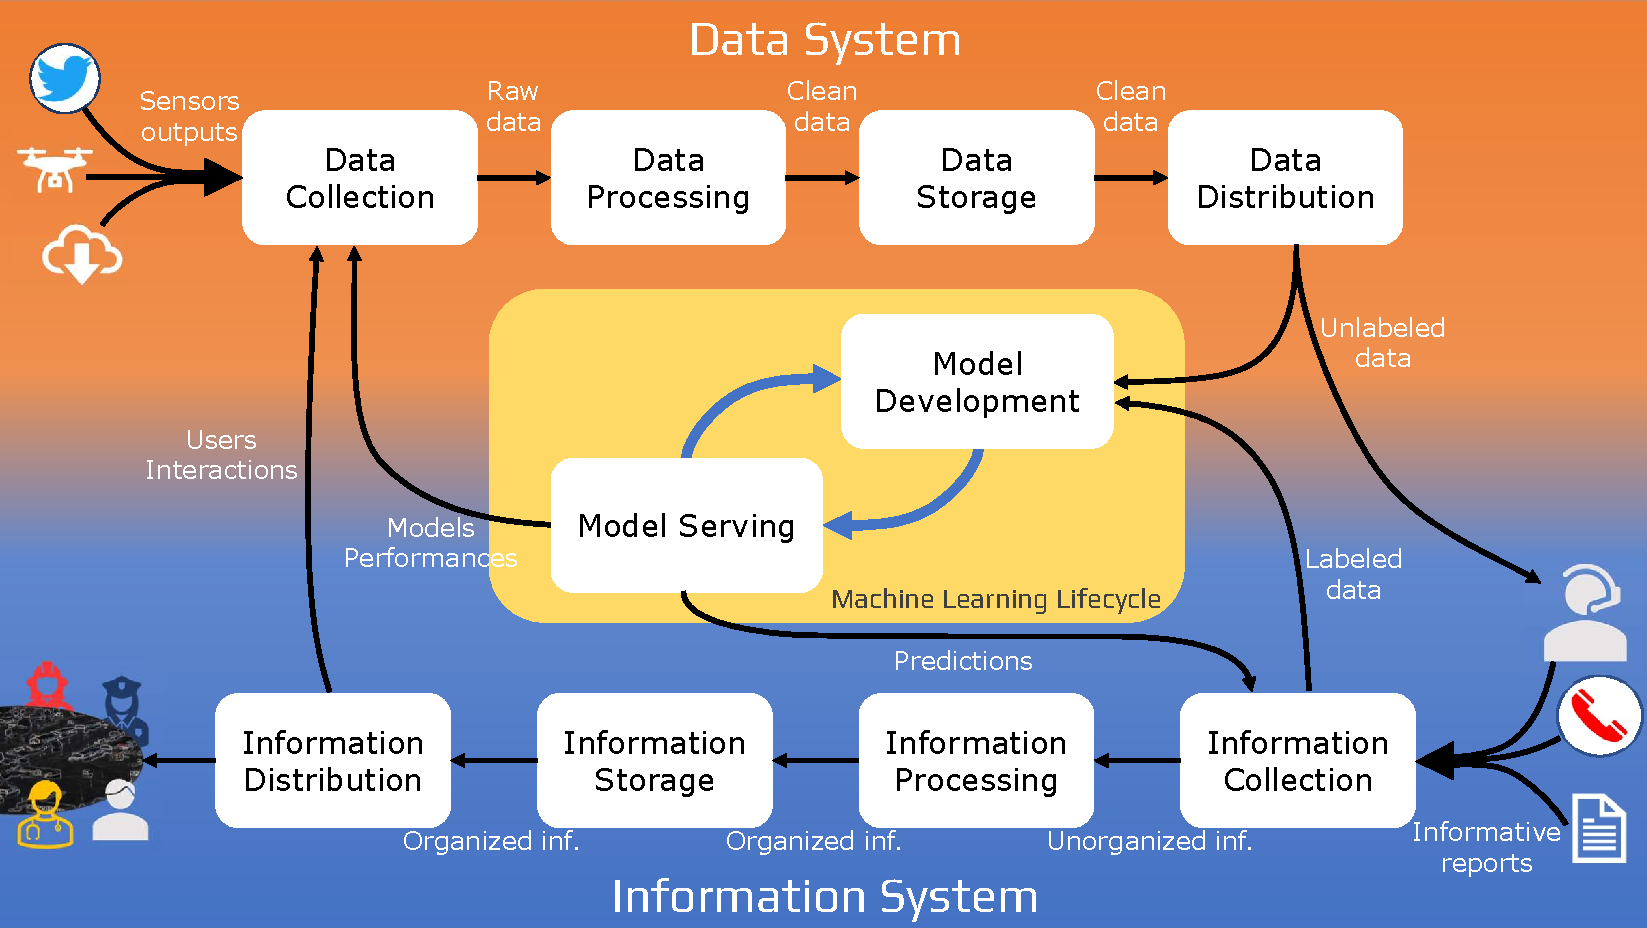
\includegraphics[width=\textwidth]{figures/chap-5/data-information-systems.pdf}
    \caption{Representation of the data system and the information system that compose a decision support system which uses machine learning models. The models are managed according to the machine learning life cycle.}
    \label{system:ds-is-systems}
\end{figure}

\subsection{The Data system}
% * Done
The management of data by a system is often considered through the 4V of Big Data \parencite{kalyvasBigDataPrimer2014}.
These 4Vs (Volume, Veracity, Variety, and Velocity) correspond to different characteristics that describe a data flow.
Given the context in which the same will be deployed, it is assumed that each V will correspond to the following:

\begin{itemize}
    \item Variety: the system is potentially expected to process a wide variety of data.
          The data expected are text messages from social media but can also be images associated with the messages, sensor readings, or drone footage.
    \item Volume: the volume of data is correlated with the sources of data.
          If the Data System only processes text messages and sensor data, the load can be expected to be standard and not require further actions.
    \item Velocity: Data are produced in real-time by the sources, and the resulting information is expected in near real-time.
          Hence, the latency induced by the processing should be kept as low as possible.
    \item Veracity: The veracity is highly variable in this context and is directly related to the data source.
\end{itemize}

The data system is responsible for managing the data that the machine learning models used to provide information and giving some indicators to the end-users.
In the former case, its role is twofold.
First, it manages the data used to train the models if they need to adapt to an ongoing event.
Secondly, it provides the models with live data.
Therefore, the data system is composed of four components, similar to the information system:

\begin{itemize}
    \item Data collection
    \item Data processing
    \item Data storage
    \item Data distribution
\end{itemize}

Each component is presented individually in the next subsection.

\subsubsection{Data Collection}
% * Done
This component is responsible for the connection with the different data sources.
It consists of a data broker such as Apache Kafka~\footnote{https://kafka.apache.org/}, that handles the different data sources.
In the case of data collection through social media, it is done through public APIs made
available by the platforms.
The platforms provide the data according to a list of terms or topics designated by the users.
Messages that contain the keywords or the topic are then returned or streamed back to the user.
As mentioned earlier, there are multiple sources of data able to provide data to the system automatically:

\begin{itemize}
    \item Social media posts
    \item Sensors (IoT: water levels, houses)
    \item Drones footages
\end{itemize}

This part acts as a gateway with the data sources.
The main issue of this component echoes the previous sections on data quality.
It may be tempting to connect to automated data sources because of their ease of access.
However, a prior study must be conducted to understand the quality of the data provided by the source.
This allows evaluating the relevance of the data provided and handling it with appropriate processing specific to the source.

\subsubsection{Data Process}
% * Done
After data collection, they are in a "raw" state.
The data must be processed to match the format expected by the rest of the system.
This component corresponds to the preprocessing step mentioned in the machine learning life cycle (Figure~\ref{system:ml-life-cycle}).
Again, this processing is typically done in two steps to ensure that the machine learning part fulfills its objectives.
First, during the preparation phase of the crisis management, the preprocessing to be performed is decided according to the data source.
Once this part is completed, the automated processing can be used during a crisis situation.
This processing is specific to the source of the data.
For example, the preprocessing of messages from Twitter and Facebook is not exactly identical.
Twitter introduces special features in the messages (RT, URLs, user mentions, etc.) that need to be processed.
The preprocessing of images and text is also different.
As mentioned in the introduction, this preprocessing is often done sequentially on the data.
Thus, using the example of Twitter and Facebook, parts of the processing pipeline can be pooled.
Therefore, this component corresponds to a catalog of preprocessing methods associated with data sources and models.
This data can then be stored or used as input for the machine learning models through the distribution component.

\subsubsection{Data Storage}
% * Done
Data storage is performed following the data policy of the organization.
Some data may not be stored for privacy reasons.
The purpose of this component is to store the data in two types of databases, depending on the usage.
A "hot" database is used during the event.
It provides indicators to the decision-makers and feeds the model training with specific data.
The second "cold" database accumulates data used during the feedback and will allow the system to be adjusted for future events.

\subsubsection{Data Distribution}
% * Done
This component is another data gateway oriented towards the consumption of the data.
The data are distributed similarly to the data sources from which they come.
The different components of the information system or the machine learning life cycle can request data according to their needs.
Unlike information, the previous steps do not prepare the data for direct consumption by decision-makers.
The data can be aggregated to provide indicators such as the volume of data flow handled by the system.
It can also feed the next component, the information collection, with unlabeled data, which external agents then label.
However, this data is primarily used to feed the machine learning models.
It can be used to make predictions and provide information to the decision-maker.
They can also be used for supervised or unsupervised training of models.

\subsection{The Information system}
% * Done
Information systems are already used by crisis management organizations.
They make use of the data collected to provide information to decision-makers.
As mentioned earlier, it is composed of four parts: Collection, Processing, Storage, and Distribution.
Similarly to the Data system, each part is described.

\subsubsection{Information collection}
% * Done
Information acquisition is, by design, one of the roles of IS.
One of the system's interfaces allows users to enter information.
Many information can be logged in the system during disaster response.
Phone calls, handled by call takers, are one instance of such information.
Using systems such as the CAD system in the US, call takers can enter the answers to the
Six W's they obtain.
The calls illustrate the definition of information provided previously.
They correspond to data that, associated with other pieces of data to create a context, possess a meaning and a value to the recipient.
Another example of information that can be entered in the Information System is the reports from emergency teams dispatched on the different hotspots of the event.
Other similar reports (weather forecast, specialized services, etc.) also fit in this category.

In an Information System that uses machine learning models, other sources of information appear.
First, the data is annotated to train the machine learning models.
The training datasets are data collected by various types of sensors, which appropriate professionals then label.
The former create information that the machine learning model will use by organizing or contextualizing the data points with associated labels.
Finally, the predictions of the machine learning models are also a source of information.
This information is then processed in the next step.

\subsubsection{Information processing}
% * Done
The information can be processed in different ways.
First of all, they can be enriched using metadata associated with the documents entered.
This metadata can then be used to organize the different information present in the system.
This organization can be hierarchical, i.e., some documents can have a higher value or priority than other documents.
The information entered can also be associated with other information already present in the system.

\subsubsection{Information storage}
% * Done
Once information is organized in the processing stage, it is stored.
The challenges faced in this component are similar to the data one.
Historically, an information system stores data organized in databases, mostly relational.
It is the organization of this data by these databases that brings information.
However, here again, machine learning brings specificity.
Indeed, the predictions made by a model can be perceived either as data or as information.
The latter case is allowed if the prediction is linked to the data initially provided to the model.
This last information is often sought in practice by the users of such systems for reasons of traceability or transparency.
In the first case, the predictions made can then be investigated after the event to improve the knowledge of the event.

\subsubsection{Information distribution}
\label{sec:information-distribution}
% * Done
Information distribution is the purpose of an information system.
It corresponds to the interface proposed to the decision-makers, such as the Common Operational Picture.
It calls also be provided along with data to provide insights from data obtained from data sources.
The output of machine learning models is directly or indirectly used at this step.
This step is crucial, as it is where all the value is delivered.
Therefore, this component can be seen as the "value bottleneck" of the information system.
As already mentioned in the previous chapters, adequate information has to be delivered to the right person at the right time.
Missing one of these conditions hinders the efforts realized in the previous steps.
The last section of this chapter elaborates on this aspect.
Finally, as just mentioned, the output of the models and users' interactions with the system can be considered data sources.
Thus, this component is looping back to the data collection component.

Previously designed information systems for decision support systems usually do not take into account the importance of data.
With the current development of machine learning methods, more and more systems are
adding machine learning models or complex analysis tools to their toolbox to always provide more insights into the situation.
This section has argued that future systems should consider two systems: one
dedicated to the organization of data and another dedicated to the organization of information.
At the interface of these two systems lie the machine learning models.
Similar to data and information, these models have their proper life cycle, as presented below previously.
This framework for organizing data and information around machine learning models is used
in the proposal presented in the next section.

\section{Case study: integration of social media in the RIO Suite software}
% * Done
\textit{R-IO Suite is introduced Section~\hyperref[sec:academic-domains]{1.4}.}

The R-IO Suite software is an information system that combines a variety of tools.
It is designed to support collaboration between actors from different organizations.
The software itself is organized around an information model that describes the collaboration between the actors.
The previous section presented a framework for designing information systems based on machine learning methods.
It allows us to question past developments and to think about new development opportunities for future information systems for crisis response.
This section presents how this framework was applied in developing the social media module of the R-IO Suite software.
The following subsection presents how the previously proposed framework fits into the crisis management framework.
In a second step, the software architecture of R-IO is briefly explained to explain how our proposal fits into this system concretely.

\subsection{Information system processes in crisis management}
% * Done
An information system such as the one presented above is intended to support the response to a disaster.
However, it takes place as a major component in the crisis management organization.
This section presents its life cycle during the different phases of crisis management to better understand the stakes of its operation.
The following three phases are considered: i) Preparation, ii) Response and iii) Recovery.
The system presents functionalities mainly for the Preparation and Response phases.

The most relevant data are used to train the machine learning models during the preparation phase—model training \& model evaluation.
They are then tested by the operators, who can then familiarize themselves with the model preparation tool.
Their feedback is taken into account to improve the interface and the predictions.

When an event occurs, the system enters a more active phase.
The system then records the data and information related to the event to quickly better understand the situation—data collection.
The data system then receives the data from the different recorded sources (social media, sensors, drones etc.).
This data is then processed—data processing—before being stored in a database—data storage.
The data in the database is then provided—data distribution—to the different actors who need it, namely:

\begin{itemize}
    \item The entry of machine learning—model deployment in the ML lifecycle.
    \item The actors who will label the data, such as specialized call center operators or citizen—information collectors.
    \item Semi-supervised or unsupervised machine learning models, if they are re-trained during crisis—model training in the ML lifecycle.
    \item Decision-makers, in the case of aggregated indicators or video data—information distribution.
\end{itemize}

These data feed different parts of the information system.
The latter is in charge of collecting the different information that appears during the disaster.
They can come from two sources: humans or computers.
In the first case, it is the information entered by the users of the system.
This can be information obtained from phone calls, reports from the teams deployed in the field, decisions made, or data tagged by volunteers.
In the case of that system, the second source of information is the pool of machine learning models that make predictions on input data.
The information thus obtained is then organized and stored in a database—information storage.
Finally, the information is provided to the decision-makers through a dedicated interface.
This interface highlights the information coming from the machine learning algorithms and, if possible, accompanies it with a relevance indicator.

During the event, a model may provide too far from initial expectations—model monitoring.
The model in question can be put into maintenance—model maintenance—and re-trained using freshly collected data to reduce the difference between its predictions and reality.
If the model is supervised and does not have sufficient labeled data for re-training, the system warns the user, who can then confirm or not the re-training.
The next section presents the software architecture of R-IO to describe better how the activities described in this section take place computationally.

\subsection{R-IO Suite Architecture}
% * Done
\begin{figure}[htb]
    \centering
    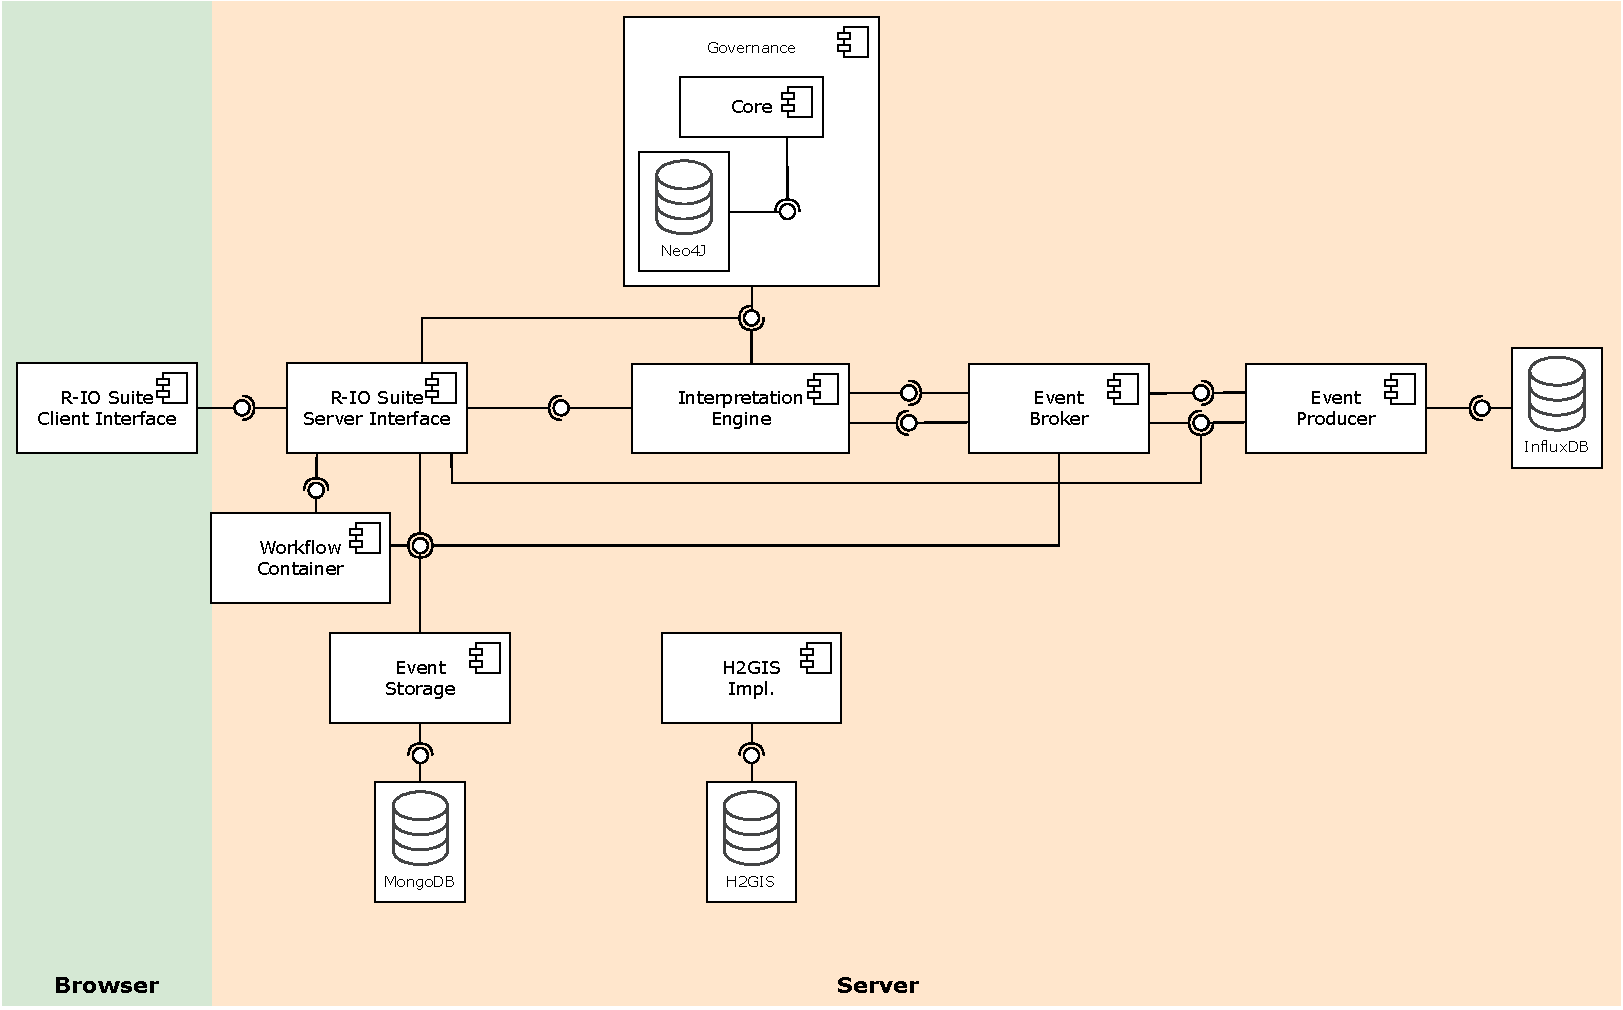
\includegraphics[width=\textwidth]{figures/chap-5/RIO-archi.pdf}
    \caption{Representation of the different components of the RIO Suite software architecture.}
    \label{system:rio-archi}
\end{figure}

R-IO is based on an event-driven architecture.
The different components are shown in Figure~\ref{system:rio-archi} and presented in the rest of this section.
RIO suite is composed of a client part and a server part.
The client part is in charge of providing the interface to the users through a Web browser.
It gets the data and information it needs from the server.
The client ensures the distribution via the display and the collection of the information provided by the users.
The server takes care of the processing and storage of the data/information as well as the collection of the data provided by automated sources.

The client consists of a single component R-IO Suite Client Interface that links directly to its server-side counterpart, the R-IO Suite Server Interface.
Both components are used to transmit data and information between the server and the client.
The server components are structured around the Event Broker.
\paragraph{Event Broker}
The Pub/Sub pattern inspires this component.
It offers an interface for the services that produce data (Pub) as well as an interface for the services that consume data (Sub).
For this purpose, the Event Broker creates subject threads in which the Pub services add their data.
The services that consume data then subscribe to the topics that interest them and consume them in these threads.
In R-IO, the Event Broker creates different threads that correspond to different events.
This component is at the heart of the event-driven architecture principle.
It is in charge of collecting data from automated sources, such as social media or sensors.
These sources then publish their data in dedicated threads consumed, mainly by the Interpretation Engine.
\paragraph{Event Storage}
The Event Storage records the various events processed by the Event Broker.
It consists of a connector to a document database (\textit{MongoDB}) that stores the events.
\paragraph{Interpretation Engine}
The Interpretation Engine processes the events that need to be processed.
It is in charge of processing information and data within the R-IO Suite software.
It contains a CEP engine made up of rules applied to the different events.
When the Interpretation Engine receives data (events), the CEP processes this data and sends it back to the Governance or to the Event Broker.
If the CEP determines that the data allows the creation or modification of an MM instance, it passes the result to the Governance and notifies the Event Broker of an event.
If the CEP only transforms the data for another use, the result is sent back to the CEP.
\paragraph{Governance}
The Governance component is in charge of the MM life cycle used by R-IO.
It has an implementation of the class model that describes the metamodel presented in Section~\hyperref[sec:crisismetamodel]{3.2}.
The classes are then implemented through different rules to orchestrate the creation, update, and deduction of instances of the MM.
The different instances then live in a graph database, \textit{Neo4J} here.
The data received by the Event Broker that is not considered events (the raw data from the data sources) are stored in a database adapted to temporal data \textit{InfluxDB}.
\paragraph{Event Producer}
This data is stored through the Event Producer, which, like the Event Storage, is an interface to the \textit{InfluxDB} database.
This component also allows to "replay" an event and its associated data by retrieving the data and calling the Event Storage.
These events are then provided to the Event Broker as a data source, allowing them to perform a simulation in a training context.
\paragraph{Workflow Container}
These training scenarios are orchestrated by the Workflow Container, which takes care of the underlying processes.
\paragraph{H2GIS Implementation}
The last component is the H2GIS Implementation, which is an interface to an \textit{H2GIS} database.
This database contains different geographical data made available for the cartographic representation provided to the user.
The next subsection describes how the elements of the architecture can be adapted to support the components of the previous framework.

\subsection{Adapting R-IO to embed machine learning models for its processing}
% * Done
\begin{figure}[htb]
    \centering
    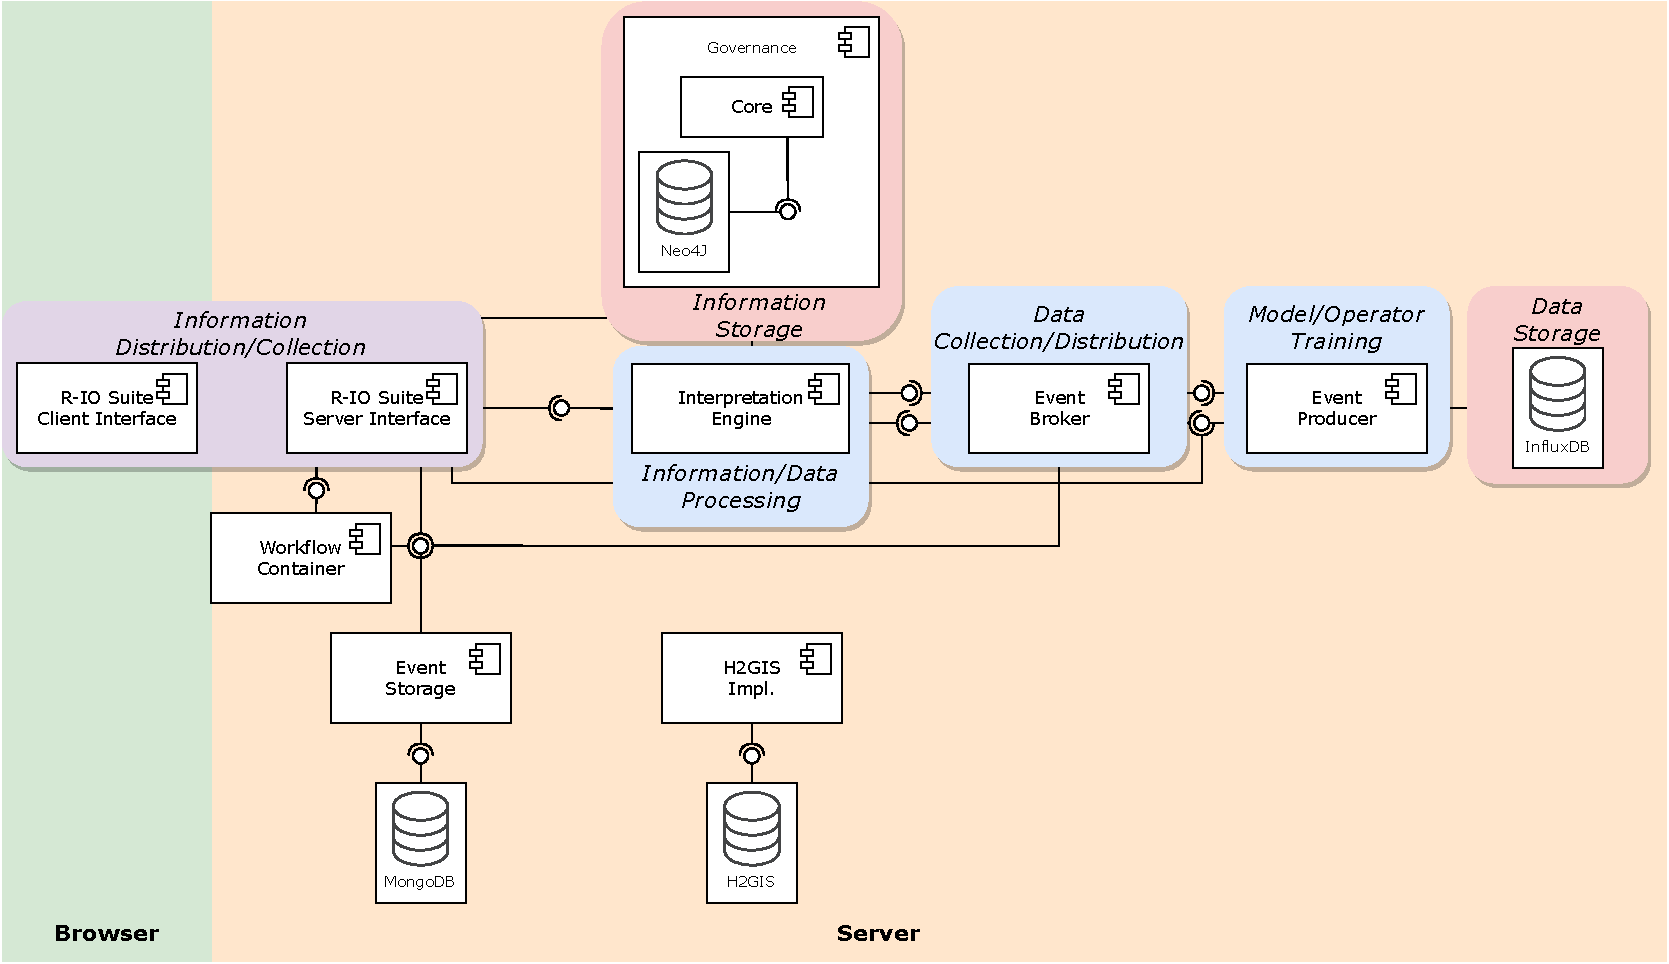
\includegraphics[width=\textwidth]{figures/chap-5/RIO-archi-concepts.pdf}
    \caption{Representation of the role played by each components of the RIO Suite software according to the data system/information system framework.}
    \label{system:rio-archi-contribution}
\end{figure}

Initially, the information contained in R-IO is processed through a Complex Event Processing engine.
The addition of the social media data processing capability leads to new needs.
First, the system now requires a capacity to manage the data collected and processed.
Secondly, to be able to process this new data, mainly using machine learning methods and models.
Integrating machine models into the operation of R-IO requires taking into account its event-driven architecture.
This section describes to what extent which component is impacted by this input.
Indeed, each function of the proposed framework Figure~\ref{system:ds-is-systems} has to be integrated.
In addition, a way to automatically manage the life cycle of the machine learning models used is also integrated.
The contribution of each software component in the data system/information system framework is represented in Figure~\ref{system:rio-archi-contribution}.
This section presents first the components related to the data system, then the components involved in the information system, and finally, the management of the life cycle of the machine learning models.

\subsubsection{Data System Integration}
\paragraph{Data Collection}
The collection of data from automated sources relies on the Event Broker.
The first step is to add the ability to connect to the various social media APIs chosen.
The data provided by the social media is then populated with threads dedicated to each source.
This data must then be processed to be cleaned.
\paragraph{Data Processing}
The Interpretation Engine is the component in charge of processing in the architecture.
Therefore, this component, which acts as a data consumer, must be equipped with various data processing methods, particularly textual ones.
Thus, depending on the thread consumed by the Interpretation Engine, various processing methods can be used.
In this way, it is possible to compose different ways of preprocessing the data depending on the original source.
This allows to mutualize this part of the architecture and to simplify the processing, as described in the introduction of this chapter.
The Interpretation Engine then sends the cleaned data to the Event Broker in a new thread, distinct according to the original data.
\paragraph{Data Storage}
This data can then be consumed by the Event Producer, which stores it in the InfluxDB database.
\paragraph{Data Distribution}
The advantage of the Event Broker is that it allows the data to be equally distributed to the various services that subscribe to the feed consumed by the Event Producer.
The data can be consumed in at least four different ways.
First, it can be served to users.
This data is then consumed by the R-IO Suite Server Interface, which passes it on to the R-IO Suite Client Interface.
They will then be consumed as metrics by decision-makers or labeled by volunteers.
This latter case is further developed in the Information Collection paragraph.

The other two ways concern machine learning models, which use the data to train or make predictions.
In the latter case, the data can be consumed by one or more machine learning models to provide predictions.
The data ready to be stored is then provided as input to the machine learning models.
These models live in the Interpretation Engine, which is the component in charge of processing.
A part of the Interpretation Engine must therefore be dedicated to data processing by machine learning models (Model Serving).
The role of this module is to provide predictions from the data provided to it.
The machine learning module is composed of several models that each corresponds to a different task.
For instance, this module can be composed of a model that identifies if:

\begin{itemize}
    \item a text message is related to a disaster event;
    \item the message is posted by a direct eyewitness of the event;
    \item geographical information is mentioned in the text;
    \item relevant information to the decision-makers are contained.
\end{itemize}

Its predictions will be provided to the CEP, in charge of determining the creation or not of new instances of the metamodel in the Neo4J database.
The predictions are then reported to the InfluxDB database, together with the original data.
The training of the models and their life cycles are described in the last part of this section.

\subsubsection{Information System Integration}
\paragraph{Information Collection}
As R-IO is an information system, users can input information through its Client Interface.
One type of information of interest is labeled data.
Interaction with the models is of the utmost importance to keep the users engaged with the model's output.
One way is to make the users decide what kind of information they want to obtain.
Of course, extensive data labeling by social media operators is not permitted in the context of disaster response.
Models, such as the one presented in chapter 4, require labeling a small set of data and should be preferred.
Currently, R-IO lacks a dedicated interface in the Client Interface to interact with machine learning models and data labeling.
Thus, it is a feature that should be integrated.
Also, as mentioned extensively in the previous sections, this part is crucial and should require extra care.
Ideally, it should be tested and iterated through the feedback of practitioners.
Once the data are transferred to the Server Interface, data are transferred to the Event Broker in a thread dedicated to labeled data.
Two components then consume this thread, the Event Producer, which updates the corresponding data in the database, with the labels attributed.
Information collected through this interface is then
\paragraph{Information Processing}
The Interpretation Engine can be seen as composed of two components.
A "low" one, which processes data and serves machine learning models, and a "higher" one, in charge of processing the information contained in the system.
The "high" level Interpretation Engine is composed of the Complex Event Processing engine that receives the information collected by the system as input.
This component analyzes predictions from machine learning models, aggregation of sensor data, and operator entries inputs.
The Complex Event Processing engine needs to be adapted to fit with the
Incoming information is then used to instantiate the different concepts of the R-IO information model.
\paragraph{Information Storage}
The Complex Event Processing Engine outputs correspond to different "instructions" sent to the Governance component.
This component then creates, updates, or deletes the corresponding instances of the information model classes that live in the Neo4j database.
The data attached to the information is published to the Event Broker, who makes it available to the Event Producer for storage.
\paragraph{Information Distribution}
Finally, the resulting information is provided to the decision-makers through the Client Interface.
Currently, a component of the Client Interface, called R-IOPLAY, is in charge of the main interface: a Common Operational Picture.
R-IOPLAY displays the different concepts of the information model geographically (see Figure~\ref{context:cop}).
This component is powered by the information models present in Neo4J, the data within the InfluxDB database.
The geographical information is provided by the H2GIS database, which is populated regularly with information available on Open Street Map.
However, R-IOPLAY does not provide other information, such as summaries of critical text messages identified or pictures identified on social media.
This part needs to be refined to be adapted to reflect the various formats of data and information that R-IO Suite handles.
The final component that requires attention is the management of the lifecycle of the machine learning models.

\subsubsection{Machine learning models lifecycle management}
%? Machine learning lifecycle
\begin{figure}[htb]
    \centering
    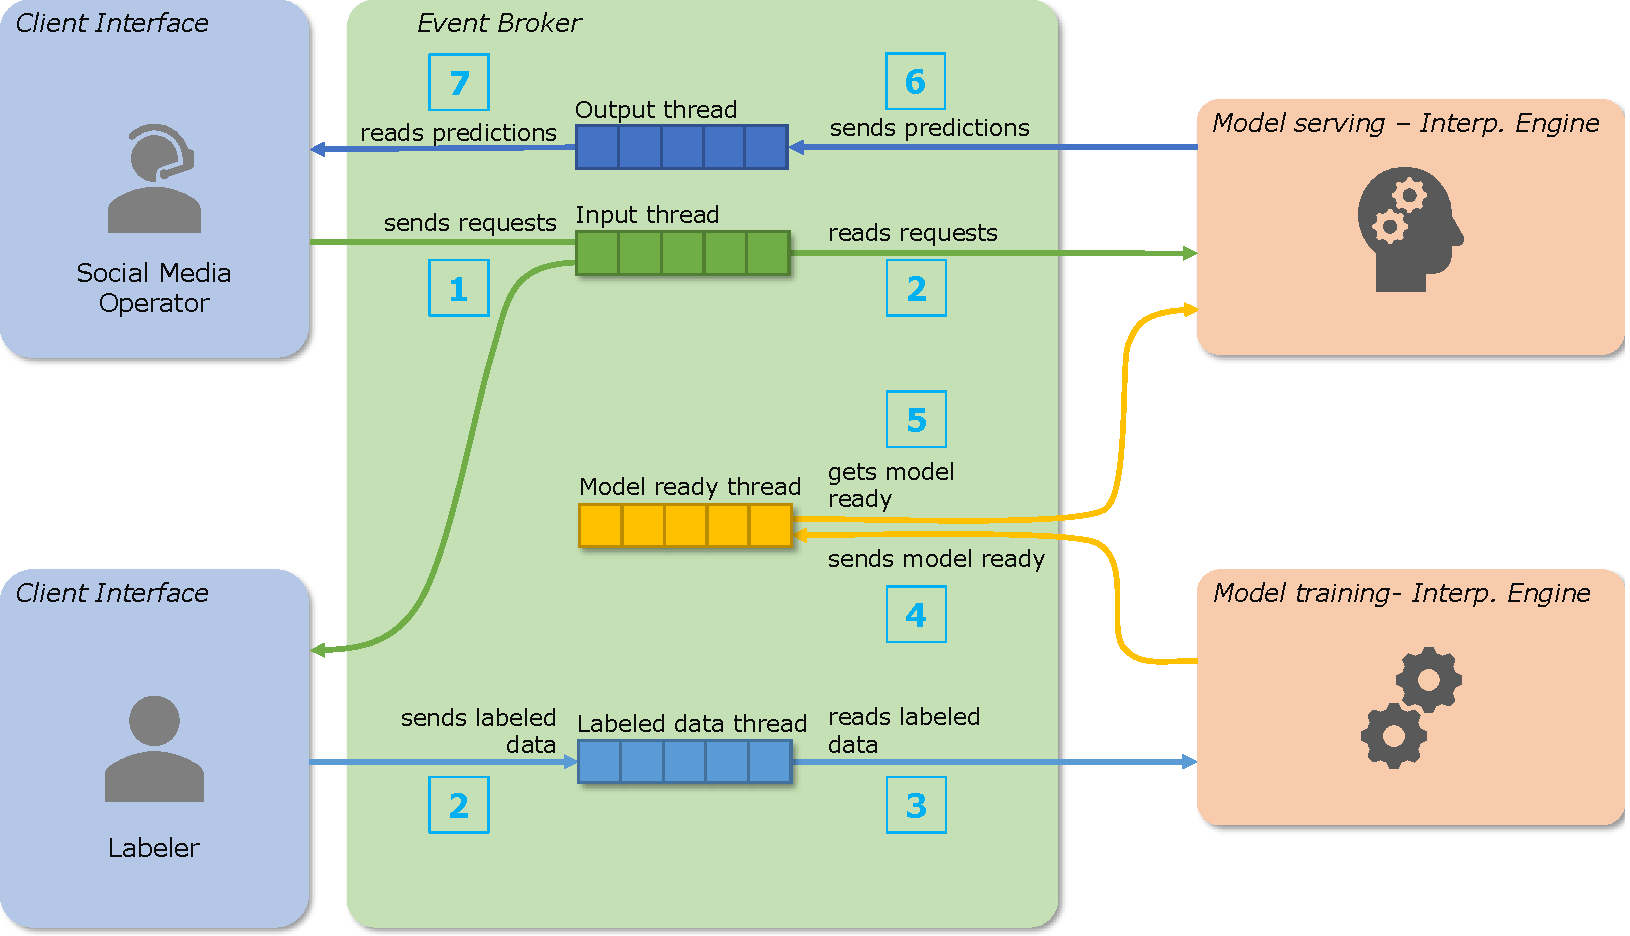
\includegraphics[width=\textwidth]{figures/chap-5/rio-ml-lifecycle.pdf}
    \caption{Illustration of model maintenance within R-IO using the Event Broker. Illustration adapted from \textcite{burkovMachineLearningEngineering2020}}
    \label{system:rio-broker-ml-lifecycle}
\end{figure}

The previous section described how the Interpretation Engine would be adapted to serve the models and make predictions from incoming data.
However, this component must also be adapted to maintain the deployed machine learning models.
This component will consist of a new module within the Interpretation Engine—the maintenance module.
Model maintenance consists essentially of a few steps.
First, identify if the model needs to go into maintenance.
Then, re-train the model with new, labeled data.
Put the model back into production so that it can make predictions again.
These different steps are orchestrated using the Event Broker.
Figure~\ref{system:rio-broker-ml-lifecycle} illustrates the process of model maintenance using the Broker.
When either the user or the module containing the model indicates to put the model in maintenance mode, an event is provided to the Event Broker.
The Event Broker then triggers the maintenance module within the Interpretation Engine, which takes care of the re-training.
The Event Broker asks the Event Producer for the labeled data it has.
The maintenance module consumes the data available to re-train the model.
Once the training is completed, the model is added to the Event Broker.
If the re-training of the model does not influence other models, the model can then be redeployed directly.
If other models depend on the re-trained model, they are re-trained in turn using the same procedure.
When all the required models are ready, they are redeployed.
This section presented a framework to organize the processing of social media data by machine learning models in an information system dedicated to crisis management.
To illustrate its functioning, the last part presented its implementation in the R-IO Suite information system.
However, although information systems for crisis management are regularly progressing, they remain the only tools within the crisis management organization.
The final section of this chapter discusses issues beyond the information system, including how its results are interpreted.

\section{Beyond the system}
% TODO Add insights from Rob Roleplay
%  ? \textcite{graceRolePlayingNext2019} reports that:
%  ? \begin{itemize}
%  ?     \item Six W's and ProQA serve as interpretive frameworks during sensemaking processes.
%  ?           The authors, therefore, note that similar systems built to process social media should
%  ?           be built with that idea in mind and "for example, pre-filtering and visualizing social media data in ways that align with domain-dependent information requirements."
%  ?     \item The way information is processed ("the information processing protocol" as per the authors) is also important, and in that sense future, social media analysts should receive the call-taker's training to create a protocol as similar as possible to theirs, allowing a better fluancy between the two information processing pipeline.
%  ? \end{itemize}
An efficient information system increases the potential of an organization tenfold.
However, as stated in Section~\hyperref[sec:information-distribution]{5.2.4.4}, the added value of the information system depends on its ability to generate better decisions, and ultimately, to improve the response.
All the effort put into providing the best possible information can be wasted if users do not read or understand that information.
The first section of this chapter warned of some problems caused by not taking cognitive mechanisms into account.
These eight issues identified are essentially related to the perception induced by the system on the user.
Over
Other challenges linked to the use of machine learning models in the systems have to be considered during the design of the interface and data collection.
However, more challenges arise beyond the system.
As a result, the context of crisis response is far from optimal for the decision-maker.
\textcite{comesCognitiveBiasesHumanitarian2016} studied the consequences of this environment on decision-makers.
Their main finding is that the crisis conditions reinforce the biases that affect decision-makers.
Biases such as conjunction fallacy or confirmation bias steer the decisions made away from the ideal set of decisions.
Users can be overly confident in the system if they are not sufficiently solicited or included in the output.
Conversely, they may not pay enough attention to the alerts it issues or the indications it provides
This last point is partly based on the trust that users have in the decision support system.
In this case, we are in a chicken and egg situation.
For the system to be adopted, it must show that it is effective, but if it is not adopted, it cannot be effective.
So the initial step must be as easy as possible to climb, bringing the interface as close as possible to what users expect to use.
This also means that they should be able to explore the limits of the system through training exercises.
Consequently, providing the correct information to the right person at the right time should not be sufficient.
The way information is received and understood should also be taken into account if one wants to build an adequate system.
Fortunately, many scholars have already explored the process of extracting sense from the information.
This process is referred to as sensemaking.
Several definitions of this process have been proposed.
For \textcite{weickSensemakingOrganizations1995}, sensemaking is the process by which individuals give meaning to their experience.
This process is retrospective—the analysis is carried out only at the end of the action.
Consequently, action is of prime importance for individuals to make sense of their environment.
The role play conducted by \textcite{graceRolePlayingNext2019} emphasizes this statement.
During their study, the authors report the importance of protocols, such as the Six W's presented in Section~\hyperref[sec:sixws]{3.1.3}.
Protocols such as the Six W's are designed to help the sensemaking of the 911 operators.
These familiar "patterns" reinforce the importance of creating a familiar mental model at the level of the system's interface and through the usage habits themselves.

\section*{Conclusion}
% * Done
This chapter considered the crisis management information system as a whole.
In particular, it was interested in the stakes of the contribution of machine learning models within an information system dedicated to crisis management.
The question originally asked was
\textit{What are the challenges faced by an information system dedicated to crisis management that uses machine learning models?}
This question was explored in three parts.
First, a review of the main feedback was carried out to understand the issues at stake for such a system.
The insights provided focused on the information system and machine learning models specifically.
The insights provided focused on the information system and machine learning models in particular.
In a second step, and considering the previous information, I proposed a framework to integrate machine learning models directly into the information system.
In this way, the predictions made by the models are associated with the rest of the information present in the system.
This framework is then applied to the R-IO Suite software to integrate social media as a data source for this software.
Finally, the last section opens on the importance of considering users and their feedback in designing and improving such systems.
This approach helps to prevent inappropriate use of the system's indications.

These observations and remarks must be considered at all levels of information system design.
From collection to distribution, the system must be thought with the context in which the user will use it.
But this remark also applies upstream when designing or choosing the algorithms embedded in the system.
Chapter 4 has already highlighted the problems posed by machine learning models in the context of disaster response.
In light of the evidence presented in those sections, algorithms over which the end-user can have influence (with proper training) appear as the option that should be preferred.
This approach can reduce the threat posed by the eight daemons identified by Endsley.
However, the benefit provided by an algorithm or a model might be deemed sufficient to be exploited.
In this scenario, extra attention is required in the design and in the interactions with the end-user to avoid the harmful consequences of opacity.
If a weakly explainable algorithm is deployed, as the benefit provided is deemed sufficient, it becomes important to reduce the friction with the user.
Taking into account these multiple observations is, however, a significant challenge.
The multitude of elements to consider implies additional cost during the design because of new constraints.

%%% Local Variables:
%%% mode: latex
%%% TeX-master: "../ma-these"
%%% End:
